\chapter{Coding}
\label{chapter:coding}

In the project's third phase, the application will be implemented as per the established specifications \cite{Hausen}. This chapter will provide a comprehensive overview of the implementation process of the application, explaining each component of the MVC architecture and providing relevant examples. Additionally, we will discuss improvements to the algorithm. The application is developed using the C++17 programming language and utilizes the following libraries throughout the development process:

\begin{itemize}
    \item OpenCV v4.5.5
    \item wxWidgets v3.2.2.1
    \item libcamera v0.0.4
\end{itemize}

Additionally, the application is developed using Visual Studio Code and CMake. A cross-compilation setup speeds up the compilation process, which compiles the code on a separate machine and transfers the compiled code to the target machine. Appendix \ref{appendix:developer-manual} provides a detailed explanation of correctly setting up the development environment and the required dependencies.

\section{View Implementation}
As discussed previously in Chapter \ref{sec:model-view-controller}, the View is responsible for displaying the data to the user. In other words,  it defines the user interface and displays the information from the model \cite{Krastev20}. In this section, the implementation of the View is discussed in detail.

To further streamline the development process of View,  a set of guidelines has been set up to be followed throughout the development process. These guidelines are as follows:

\subsubsection{Handling User Input}
This guideline emphasizes that the View should be adept at managing and processing user interactions. It is responsible for capturing user inputs, such as mouse clicks, keyboard entries, or touch gestures, and conveying them to the Controller for further processing. This can involve events like form submissions, button clicks, or interactions with interactive elements on the user interface.

\subsubsection{Avoid any business logic}
This requirement underscores the importance of maintaining a clear separation of concerns within the MVC architecture. The View should refrain from incorporating any form of business logic that involves tasks like data validation, computation, or decision-making processes. Instead, these responsibilities are delegated to the Model and Controller components. By adhering to this guideline, the View remains focused on its core function of presenting data and interacting with the user interface.

\subsubsection{Avoiding Direct Model Manipulation}
This guideline reinforces the principle of ensuring that the View does not directly modify the state or data of the Model. Instead, any alterations to the underlying data should be orchestrated through the Controller. This guideline establishes a controlled data flow within the application, maintaining data integrity and adherence to the MVC architectural pattern.

\subsubsection{Utilizing Templates or Layouts}
In the development of the View component, it is recommended to use templating engines or layout systems. These tools enable the creation of modular and reusable components that can be combined dynamically to build the user interface. By utilizing templates or layouts, developers can simplify the design and rendering of the View, leading to a more scalable and maintainable codebase.

\subsubsection{Error Handling and Feedback Mechanisms}
This guideline emphasizes implementing robust error-handling mechanisms within the View. It is important to provide clear and informative feedback to the user in case of errors or invalid inputs. This guideline guides users through the application's workflow, even when unexpected events occur. Effective error handling contributes to a more user-friendly and reliable user experience.

\subsection {Main Layout}
The implementation of the main layout is the first step in the development of the View. The main layout is the universal layout that is used throughout the application. The implementation is done based on the result of the wireframing process, which is done in Section \ref{subsec:wireframe}.

The main layout is shown in Figure \ref{fig:main_layout}. The main layout consists of the title, image, status, and button panels. All components' functions are explained previously in Section \ref{subsec:wireframe}.

\begin{figure}[!ht]
    \centering
    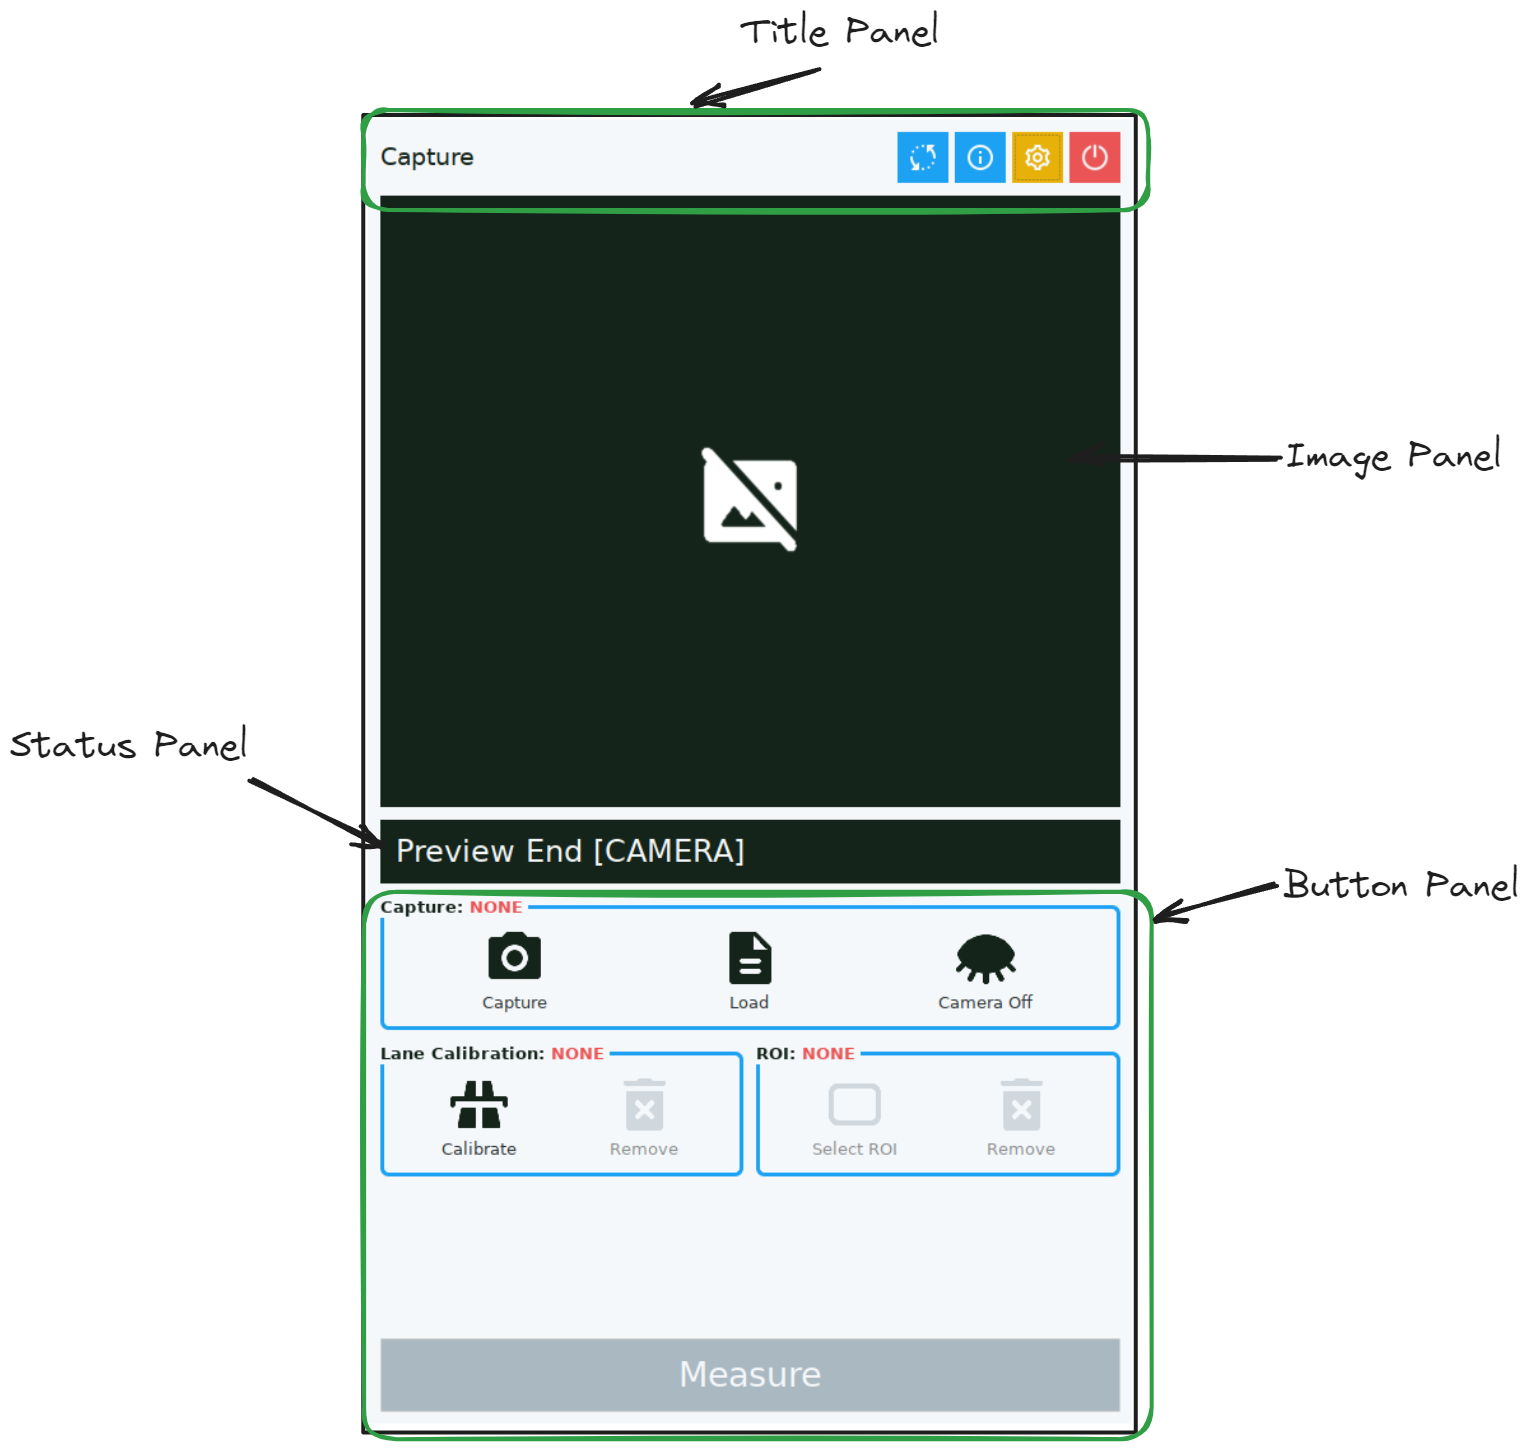
\includegraphics[width=0.45\textwidth]{texs/Part2/chapter4/image/mainlayout.png}
    \caption{Main Layout}
    \label{fig:main_layout}
\end{figure}

\begin{figure}[!ht]
    \centering
    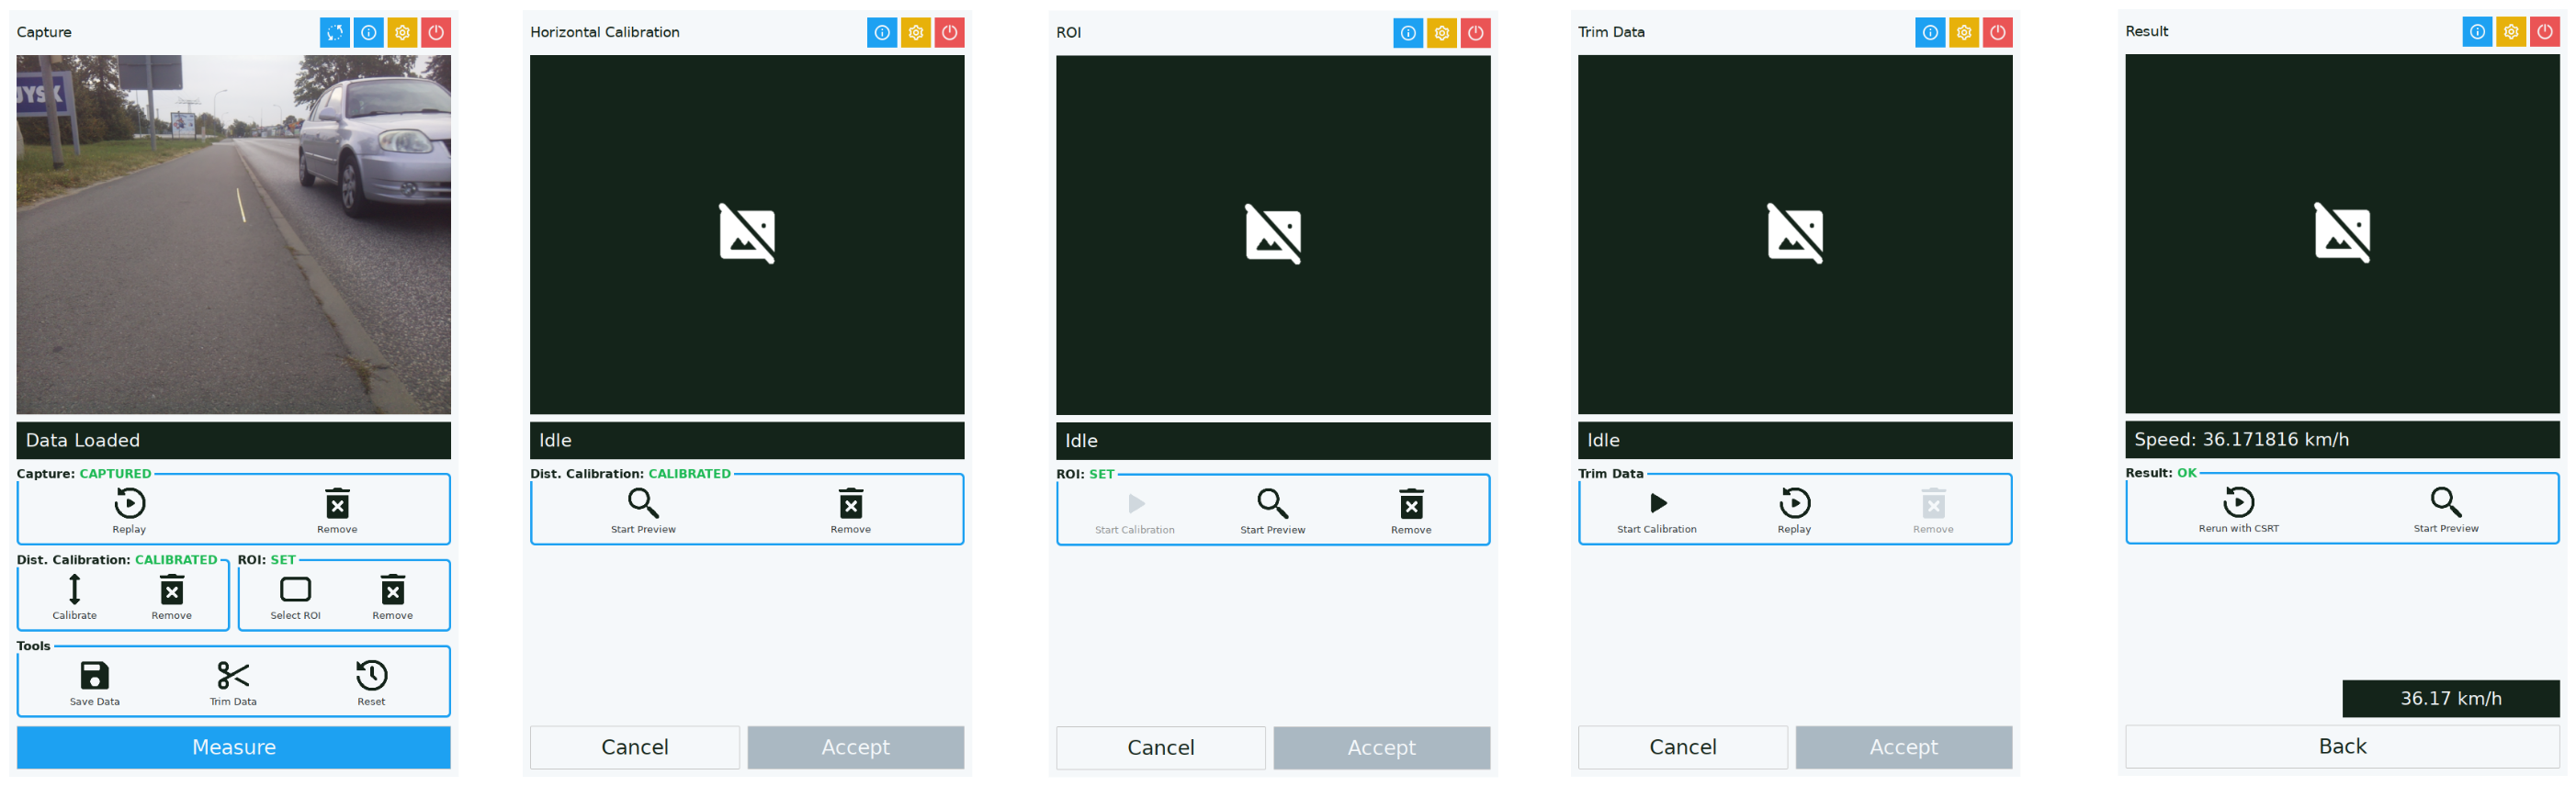
\includegraphics[width=\textwidth]{texs/Part2/chapter4/image/otherpanel.png}
    \caption{Example of other implemented Panels}
    \label{fig:otherlayouts}
\end{figure}

Figure \ref{fig:otherlayouts} shows multiple other panels used within the application. As observed, these panels all have similar layouts, with the only difference being the components within the button panels. This similarity is intentional, as it helps to maintain consistency within the application. This layout is implemented by the base class \texttt{BasePanel} and \texttt{BasePanelWithTouch}. For more details, please refer to the project documentation in Appendix \ref{appendix:documentation}.

\subsection{Button Panel}
\label{subsec:button_panel}

This panel is responsible for displaying bitmap buttons that users can interact with. Bitmap buttons are buttons that have an image as their icon. They initiate specific processes within the application, such as capturing an image or calibrating the camera. During the implementation phase, multiple types of bitmap buttons are used. Within the panel also contains group boxes, which is used to group buttons with similar functionalities. The implementation of these components is discussed in detail below.

\subsubsection{Bitmap Button}
Bitmap Button is a type of button that are used widely within the application. It contains a bitmap image and a text label positioned below the image. Figure \ref{fig:bitmap_button} shows an example of the bitmap buttons used within the application.

Throughout the implementation process, three different types of
bitmap buttons are implemented. They are Type 1, Type 2, and Type 3. Two types, Type 1 and Type 2, share a similar design concept but differ in their state handling.

\begin{figure}[!ht]
    \centering
    
\includegraphics[width=0.45\textwidth]{texs/Part2/chapter4/image/bitmapbutton.png}
    \caption{Bitmap Button}
    \label{fig:bitmap_button}
\end{figure}

Figure \ref{fig:type1_state} shows the button appearance in different states for the Type 1 bitmap button. This type of button is designed to be utilized for process that requires a long time to complete. For example, when capturing an image, the button assumes a \textit{NORMAL} state when no image has been captured. When pressed, the process started, and the button transitions to an \textit{ACTIVE} state, signifying that the process is underway. During this active state, the button is also disabled to prevent any potential interruptions or accidental re-triggering of the process. Once the process is completed, the button shifts to a \textit{DISABLE} state, preventing the reinitiation of the process.

\begin{figure}[!ht]
    \centering
    
\includegraphics[width=0.45\textwidth]{texs/Part2/chapter4/image/type1state.png}
    \caption{Type 1 Button State}
    \label{fig:type1_state}
\end{figure}

\begin{figure}[!ht]
    \centering
    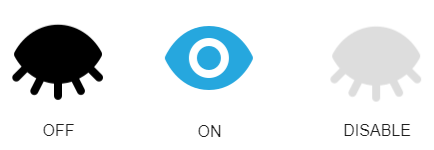
\includegraphics[width=0.45\textwidth]{texs/Part2/chapter4/image/type2state.png}
    \caption{Type 2 Button State}
    \label{fig:type2_state}
\end{figure}

The states for the Type 2 button are shown in Figure \ref{fig:type2_state}. This type of button is used when the button is used to trigger a process that requires toggling. For instance, when turning on a camera, the button assumes an \textit{OFF} state when the process has not been initiated and is available for activation. Upon pressing the button, the process initiates, and the button transitions to an \textit{ON} state, indicating that the process is actively running. If necessary, pressing the button again will revert the state to \textit{OFF}, effectively terminating the ongoing process.

\begin{figure}[!ht]
    \centering
    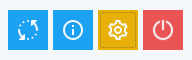
\includegraphics[width=0.45\textwidth]{texs/Part2/chapter4/image/type3state.png}
    \caption{Example of Type 3 Button}
    \label{fig:type3_state}
\end{figure}

The last type of bitmap button is Type 3. In terms of appearance, it differs from the previous two types. This button contains only a bitmap image without the text label. It does not have states and is used to handle a straightforward process, such as exiting the application or opening the settings panel. An example of a Type 3 bitmap button can be seen in the title panel (see Figure \ref{fig:type3_state}).

\subsection{Group Box}

Organizing buttons with similar functions using a Group Box is a beneficial practice that can elevate the user experience. This component can streamline navigation and improve overall functionality by grouping buttons that perform similar tasks. As an illustration, the Capture Panel (as exemplified in Figure \ref{fig:group_example}) displays three distinct groups: Capture, Calibration, and ROI. Within the Capture Group, three buttons relate to the capturing process: the Capture Button, which captures images; the Load Button, which loads images; and the Toggle Camera Button, which activates the camera.

Furthermore, the Group Box can also display the state of the application. For example, the Capture Group Box shows the current state of the captured data, whether it is empty or already captured (refer to Figure \ref{fig:group_state}). When the data is empty, the Group Box will display \textit{NONE} text in red. On the other hand, if the data is captured, the Group Box will display the text \textit{CAPTURED} in green color.

\begin{figure}[!ht]
    \centering
    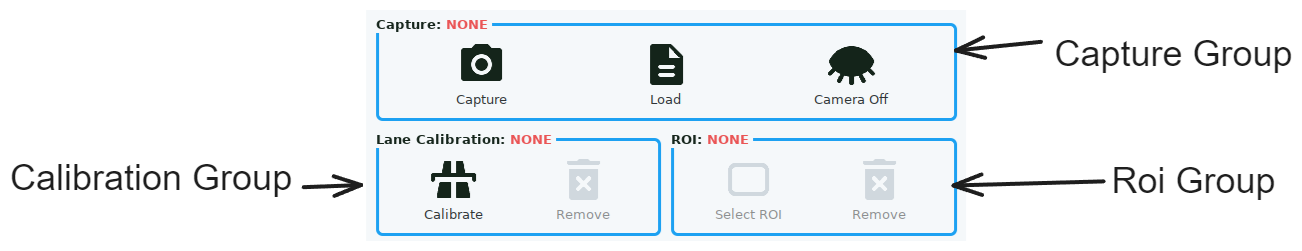
\includegraphics[width=0.75\textwidth]{texs/Part2/chapter4/image/groupexample.png}
    \caption{Groups within Capture Panel}
    \label{fig:group_example}
\end{figure}

\begin{figure}[ht!]
    \centering
    \begin{subfigure}[c]{0.8\textwidth}
        \begin{minipage}{\textwidth}
            \centering
            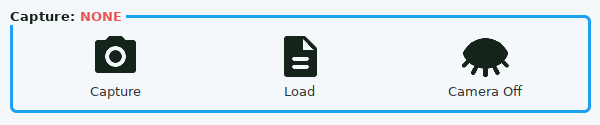
\includegraphics[height=2 cm]{texs/Part2/chapter4/image/ok10.png}
        \end{minipage}
        \caption{Data is Empty}
        \label{fig:group_empty}
    \end{subfigure}
    % \hfill
    \begin{subfigure}[c]{0.8\textwidth}
        \begin{minipage}{\textwidth}
            \centering
            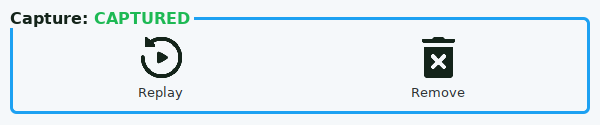
\includegraphics[height=2 cm]{texs/Part2/chapter4/image/ok11.png}
        \end{minipage}
        \caption{Data is Captured}
        \label{fig:group_captured}
    \end{subfigure}
    \caption{Example of different states of Group Box}
    \label{fig:group_state}
\end{figure}

\subsubsection{Handling Button Input}
\label{subsubsec:handling_button_input}
The button input is handled using wxWidgets' provided event mechanism. For more details, refer to wxWidgets Documentation \cite{wxWidgetsEvent}.

Handling button input involves binding the button to a specific function. When the button is pressed, an event is captured, and the function is executed. Depending on the implementation, different buttons can trigger different functions. For instance, pressing the button to turn on the camera will trigger a function to activate the camera, while pressing the button to capture an image will trigger a function to take a picture.

To assign a specific function to a button, giving each button a unique ID is necessary. This unique identifier makes identifying and linking the button to a particular function easier. Detailed instructions on binding specific buttons to a function can be found in the developer manual in Appendix \ref{appendix:developer-manual}. Alternatively, the project documentation in Appendix \ref{appendix:documentation} also provides a detailed explanation of the process.

\subsubsection{Updating Button State}
A proper feedback mechanism is essential to ensure that the user is aware of the current state of the application. In the application context, the button state is used to provide feedback to the user on the current state of the application. For example, when the user interacts with a button to turn on the camera, the feedback to the user is that the button state changes from \textit{OFF} to \textit{ON}.

Updating the button state is done using event handling, similar to the process of handling button input. An event is created and captured when an update is required, for example, after a button is pressed or a process is completed, and the button state is updated accordingly. The controller component usually does this process, as it handles the application logic.

However, it is also important to note that while updating the component state is crucial, updating it too frequently can harm the application's performance. Therefore, it is crucial to find a balance between the two.

\subsection{Image Panel}
\label{subsec:image_panel}
The Image Panel component is a crucial element of the user interface. It is a dynamic component that provides visual feedback and interactive input to the user. Its value lies in its ability to convey important information in real time to the user, providing updates on the application's state. For example, during the image-capturing process, the Image Panel displays the captured image instantly, giving users immediate visual feedback.

Moreover, the Image Panel also functions as a responsive input mechanism. Through proper event handling, users can interact with the Image Panel using various input methods, such as mouse interactions or touch-based inputs. This section focuses on the processes involved in presenting images to the user and enabling user interactions.

\subsubsection{Displaying Image to the User}
The \texttt{UpdatePreviewEvent} is a specific type of \textit{Data Event} responsible for updating images on the image panel. In general, a \textit{Data Event} is an event that contains data, which is discussed in greater detail in Section \ref{subsec:event_as_feedback_mechanism}. This event is usually created by either the Controller or threads, including the image that needs to be updated.

For instance, in displaying images from the camera within a thread's execution, every thread loop will create the \texttt{UpdatePreviewEvent} and the current camera image will also be included. The View will catch the submitted event, unpack the data, and display the information on the image panel.

\subsubsection{Handling Touch Input}
\label{subsubsec:handling_touch_input}
Input from users can be achieved through the touch input, which shares similarities with the button input. It is possible to attach touch events to a function, which will be executed whenever a touch event occurs.

The \texttt{wxMouseEvent} from wxWidgets can be utilized to enable this functionality. Alternatively, the \texttt{BasePanelWithTouch} class can also be inherited during View implementation. This class already has implemented touch event handling, including methods to handle these events. For further details, kindly refer to the project documentation in \ref{appendix:documentation}.

\subsection{Message Dialog}
\label{subsec:message_dialog}

A dialog is a user interface component commonly used in various libraries and frameworks. It is a modal window that appears on top of the application content to provide important information or ask for a decision \cite{Bay_2022}. When a dialog is open, all app functionality is disabled, and it persists on the screen until the user takes the required action, confirms it, or dismisses it \cite{Bay_2022}.

This UI component is crucial, as it can provide users when immediate attention is necessary \cite{MaterialUI}. A simple use case for Dialog is with error handling. When an error occurs, a Dialog can inform the user about the error and provide options for the user to take action and resolve the problem. Another use case is when the user needs to make a decision. For example, when the user wants to exit the application, a Dialog can be used to confirm the user's decision.

According to Android Developers \cite{Android_Developers}, A dialog box typically includes a title, some text, and buttons for users to take action. The title briefly describes the dialog's purpose, while the text provides more detailed information. Users can take action by clicking on the buttons. Figure \ref{fig:message_dialog} shows an example of the dialog component.

\begin{figure}[!ht]
    \centering
    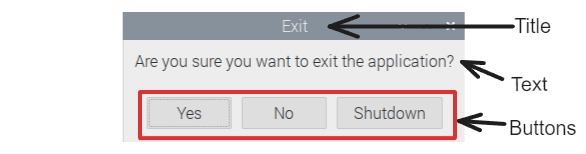
\includegraphics[width=0.65\textwidth]{texs/Part2/chapter4/image/dialog.png}
    \caption{Example of Message Dialog}
    \label{fig:message_dialog}
\end{figure}

\subsection{Navigating between different panel}
\label{subsec:navigating_between_different_panel}

This application has multiple panels or views implemented based on its different functionalities. For instance, the capture panel helps capture an image, while the calibration panel helps perform camera calibration. Since there are multiple views, it is essential to have a proper control method to display them to the user.

To simplify the process, we have implemented a rule that only one View can be displayed within the frame while the others remain hidden. The implementation is done by using the \texttt{Show()} and \texttt{Hide()} methods provided by wxWidgets. The current active View will be hidden with the \texttt{Hide()} method during the navigation process, while the new View will be shown.

An example of navigating between different panels by using \texttt{Show()} and \texttt{Hide()} methods is shown in Figure \ref{fig:show_panel}.

\begin{figure}[!ht]
    \centering
    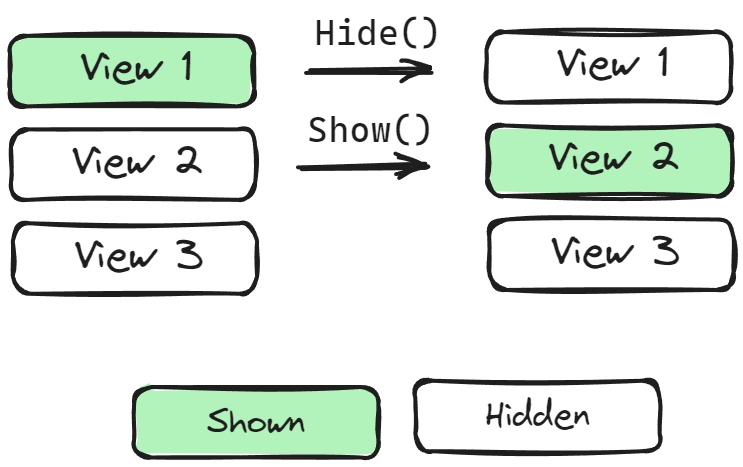
\includegraphics[width=0.45\textwidth]{texs/Part2/chapter4/image/showpanel.png}
    \caption{Example of navigating between different panel}
    \label{fig:show_panel}
\end{figure}

\section{Model Implementation}
\label{sec:model_implementation}

\subsection{Session Data}
\label{subsec:session_data}

In this section, an overview of the Session Data is provided. This component is a part of the Model, which is responsible for storing the data and the application logic. Figure \ref{fig:sessiondata_overview} shows the overview of the Session Data.

\begin{figure}[!ht]
    \centering
    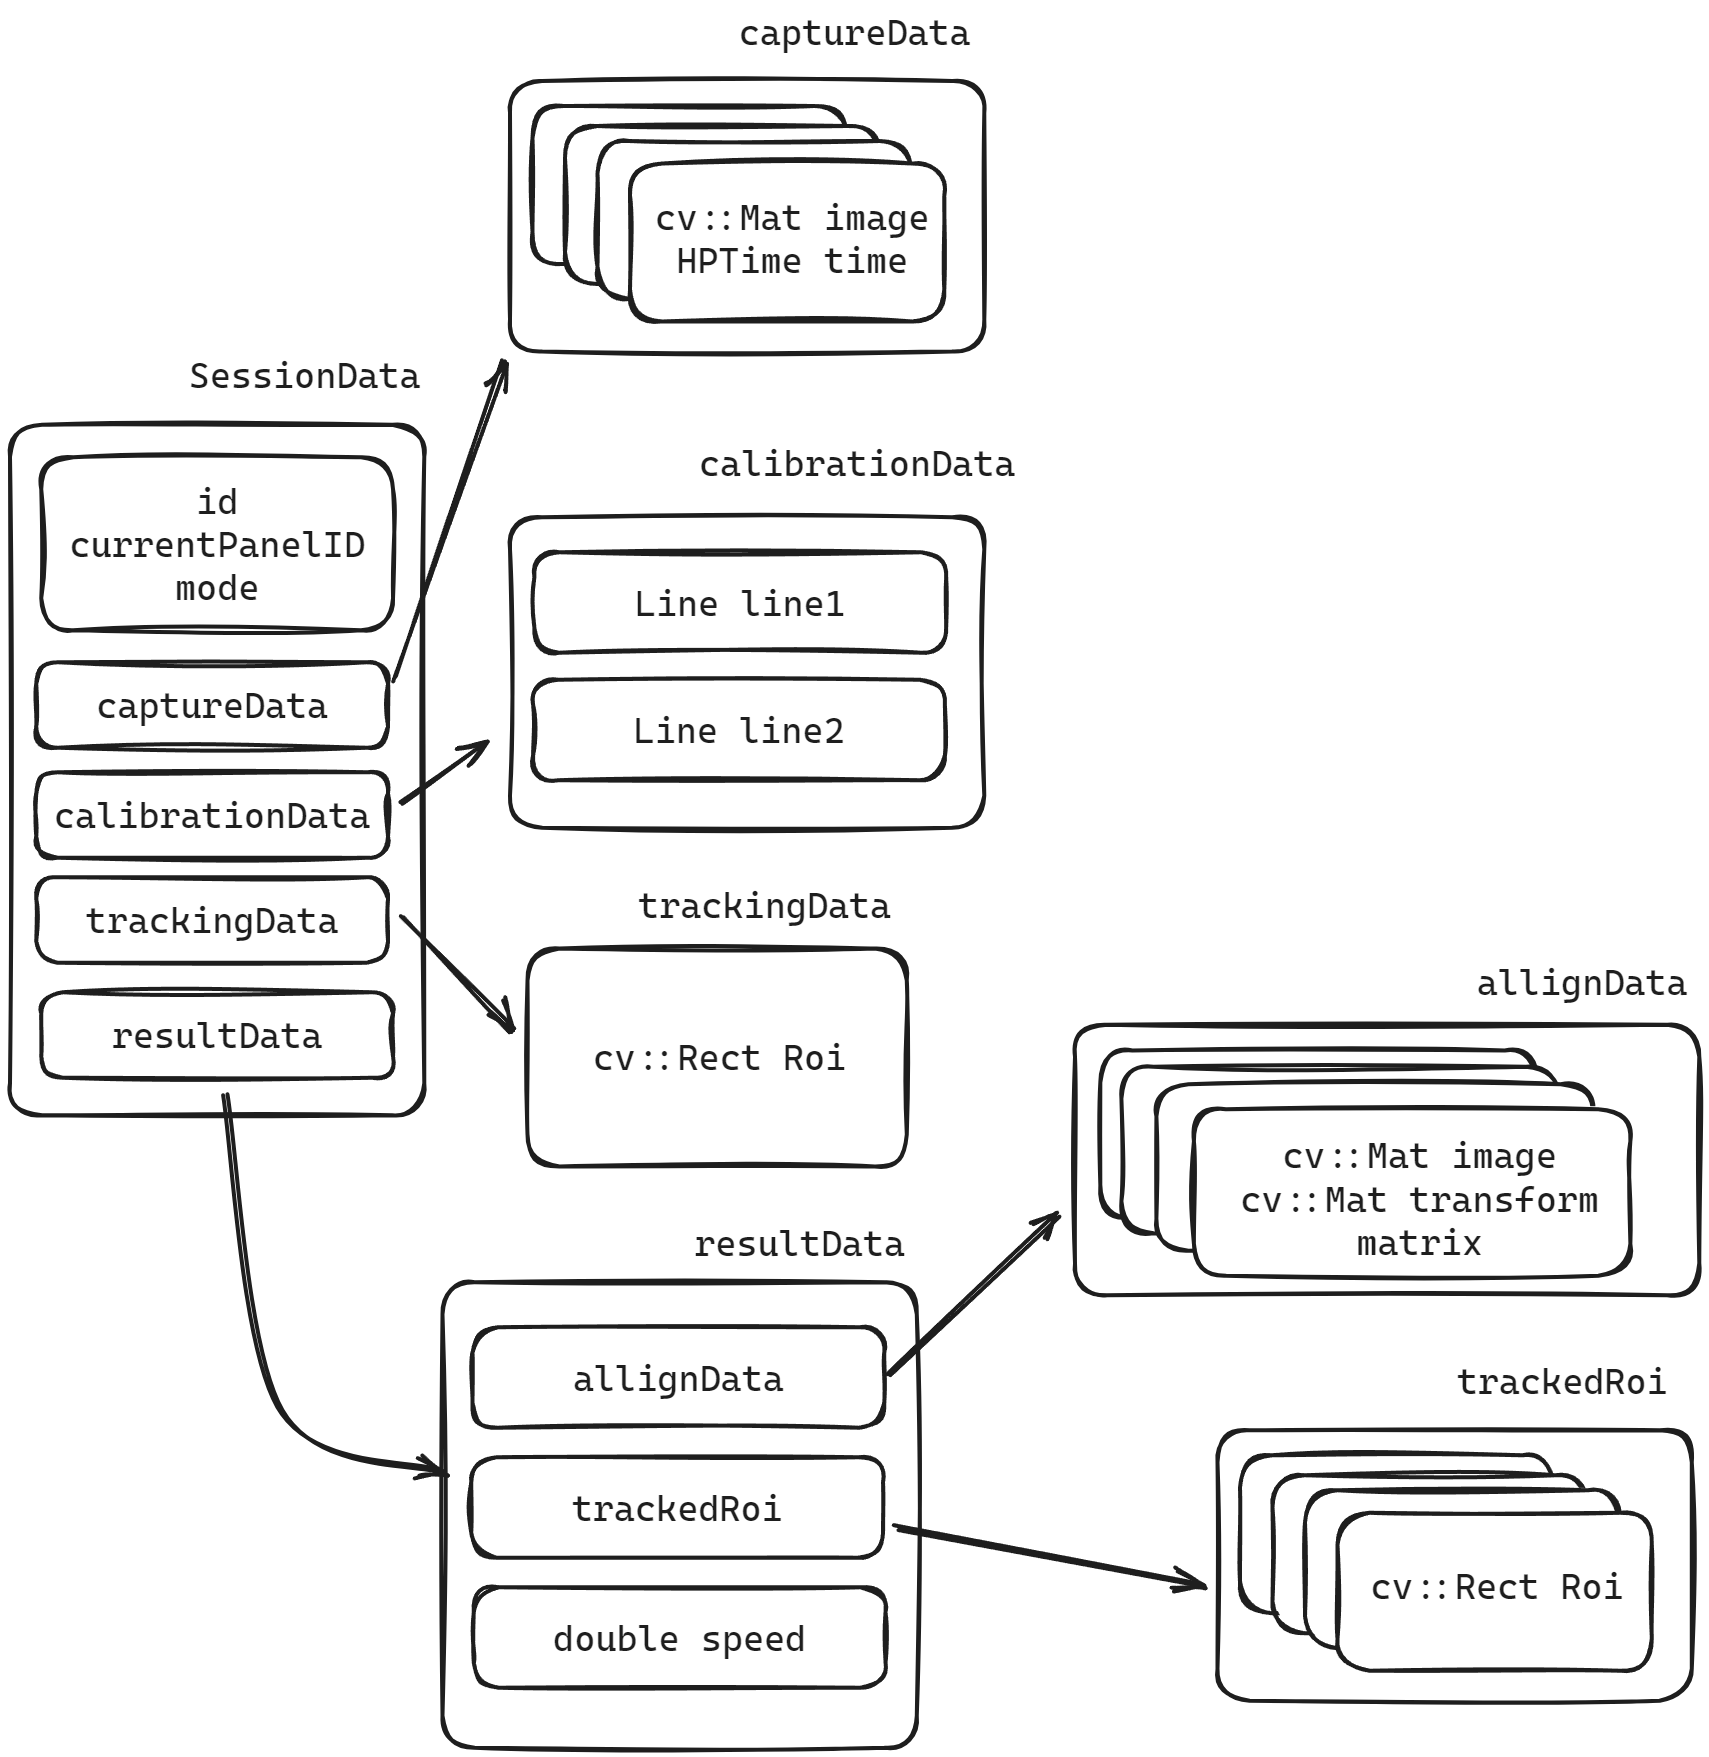
\includegraphics[width=0.45\textwidth]{texs/Part2/chapter4/image/sessiondata.png}
    \caption{Overview of Session Data}
    \label{fig:sessiondata_overview}
\end{figure}

The Session Data consists of four subcomponents, which are \texttt{CaptureData}, \texttt{CalibrationData}, \texttt{TrackingData}, and \texttt{ResultData}. Each of these components is explained in detail below.

\textbf{CaptureData:} This data stores a vector of original images captured by the camera. Alongside the image, this data type is also responsible for storing the time the image is captured to be used for measurement purposes.

\textbf{CalibrationData:} Contains the result of the calibration process, which are the variables \textit{line1} and \textit{line2}. Both of these \texttt{Line} objects represents the calibrated lines, which are required for the measurement process as mentioned in previous work \cite{Sabtu_2023}.

\textbf{TrackingData:} This data stores the initial region of interest (ROI) on which the tracked object is located. This implementation helps to filter out unwanted objects during tracking, which will helps the optical flow algorithm to focus on the tracked object.

\textbf{ResultData:} The data contains the output of a calculation process, consisting of three variables: \texttt{allignData}, \texttt{trackedRoi}, and \texttt{speed}. The \texttt{allignData} variable stores the output of the alignment process, while the \texttt{trackedRoi}variable stores the ROIs on which the tracked object is located. The \texttt{speed} variable represents the speed of the tracked object, which is calculated using the outputs of both the alignment and tracking processes.

\section{Controller Implementation}
\label{sec:controller_implementation}

As mentioned previously in Section \ref{sec:software-architecture}, each View component will have its Controller associated with it. By doing so, each Controller will have specific responsibility for handling the application logic for the View. Furthermore, this design also helps in terms of application scaling. Having multiple controllers allows the application logic to be divided into smaller parts, making it easier to maintain and scale.

However, proper controller design guidelines are required to implement these controllers properly. Therefore, we have set up a set of guidelines that we have followed throughout the development process. These guidelines are as follows:

\subsubsection{Only handle request and response}
This guideline emphasizes that the Controller should only focus on handling requests and responses between View and Model. It should not contain any business logic. Instead, the business logic should be implemented in the threads, which will be discussed in Section \ref{subsec:thread_and_thread_controller}.

\subsubsection{Provide similar endpoints}
To ensure proper communication between the Controller and the View, providing similar endpoints for each Controller is important. By doing so, developers can easily identify the communication methods between the View and the Controller. To properly implement this guideline, all methods responsible for communication between the View and the Controller should be named with the prefix \texttt{e\_}, which stands for an endpoint. For example \texttt{e\_startCamera()}, \texttt{e\_captureImage()} and \texttt{e\_calibrate()}.

\subsubsection{Only handle one view}
This guideline emphasizes that each Controller should only handle one View. This guideline ensures that the Controller is manageable with a few responsibilities, which enables the Controller to be easily maintained and scaled.

\subsubsection{Singular responsibility}
Each endpoint should only handle one responsibility. For example, \texttt{e\_startCamera()} should only handle the process of starting the camera and not other processes, such as capturing an image or calibrating the camera.

\subsubsection{Handle error}
All endpoints should be wrapped with a try-catch block to handle any error during the process. If an error occurs, an \texttt{ErrorEvent} will be created and passed to the view component. The View component will then display the error message to the user using a message dialog, as discussed previously in Section \ref{subsec:message_dialog}.

\subsubsection{Prevent handling outside active panel}
\label{subsec:prevent_handling_outside_active_panel}
This guideline emphasizes that the Controller should only handle requests and responses when the View is active. This strict rule is implemented to prevent any unwanted behavior that might occur when the View is not active. The \texttt{checkPrecondition()} provides a method to check whether the View is active. If the View is inactive, an error message will be displayed to the user.

\subsection{Event as a Feedback Mechanism}
\label{subsec:event_as_feedback_mechanism}

As mentioned previously in Section \ref{sec:software-architecture}, the Controller is responsible for handling the application logic. This process involves handling requests, which is done via the endpoints, while the responses are handled via the events.

Within this project, events play a huge role in the communication process between the View and the Controller. Events do not simply inform the View regarding the request status; they can also pass data between the View and the Controller. Hence, two types of Events are defined, which are \textit{Empty Event} and \textit{Data Event}.

\textit{Empty Event} is an event that does not contain any data. It is used to inform the View regarding the status of the request. This type of event is usually utilized to inform the user of the current status of the requested process, such as when the process is started, completed, or failed.

\textit{Data Event}, on the other hand, acts as a container to pass data between the View and the Controller. This type of event is used when the View requires data from the Model, such as the captured image or the result of the calculation process. This type of event is also used to update the View with the latest data, such as the current camera image or application state.

Creating and handling events is done using wxWidgets' provided event mechanism. For more details, refer to wxWidgets Documentation \cite{wxWidgetsEvent}. Alternatively, the Project Documentation in Appendix \ref{appendix:documentation} also explains how to create custom events.

\subsection{Threads and Thread Controller}
\label{subsec:thread_and_thread_controller}
To reduce the Controller's responsibility, handling the business logic is tasked to the \textit{threads}. Separating the execution of business logic on different threads prevents the main thread or the GUI thread from being blocked. This design decision is essential to ensure the application's responsiveness.

When a process needs to be executed, the Controller handles the request and signals the Thread Controller to initiate the process. The process runs independently on different threads, and once the task is finished, the Thread Controller is informed to close the threads. The entire process is handled through the Controller endpoint and Event.

Figure \ref{fig:sequence_diagram} provides a sequence diagram illustrating the connections of the MVC components with the Thread Controller.

\begin{figure}[!ht]
    \centering
    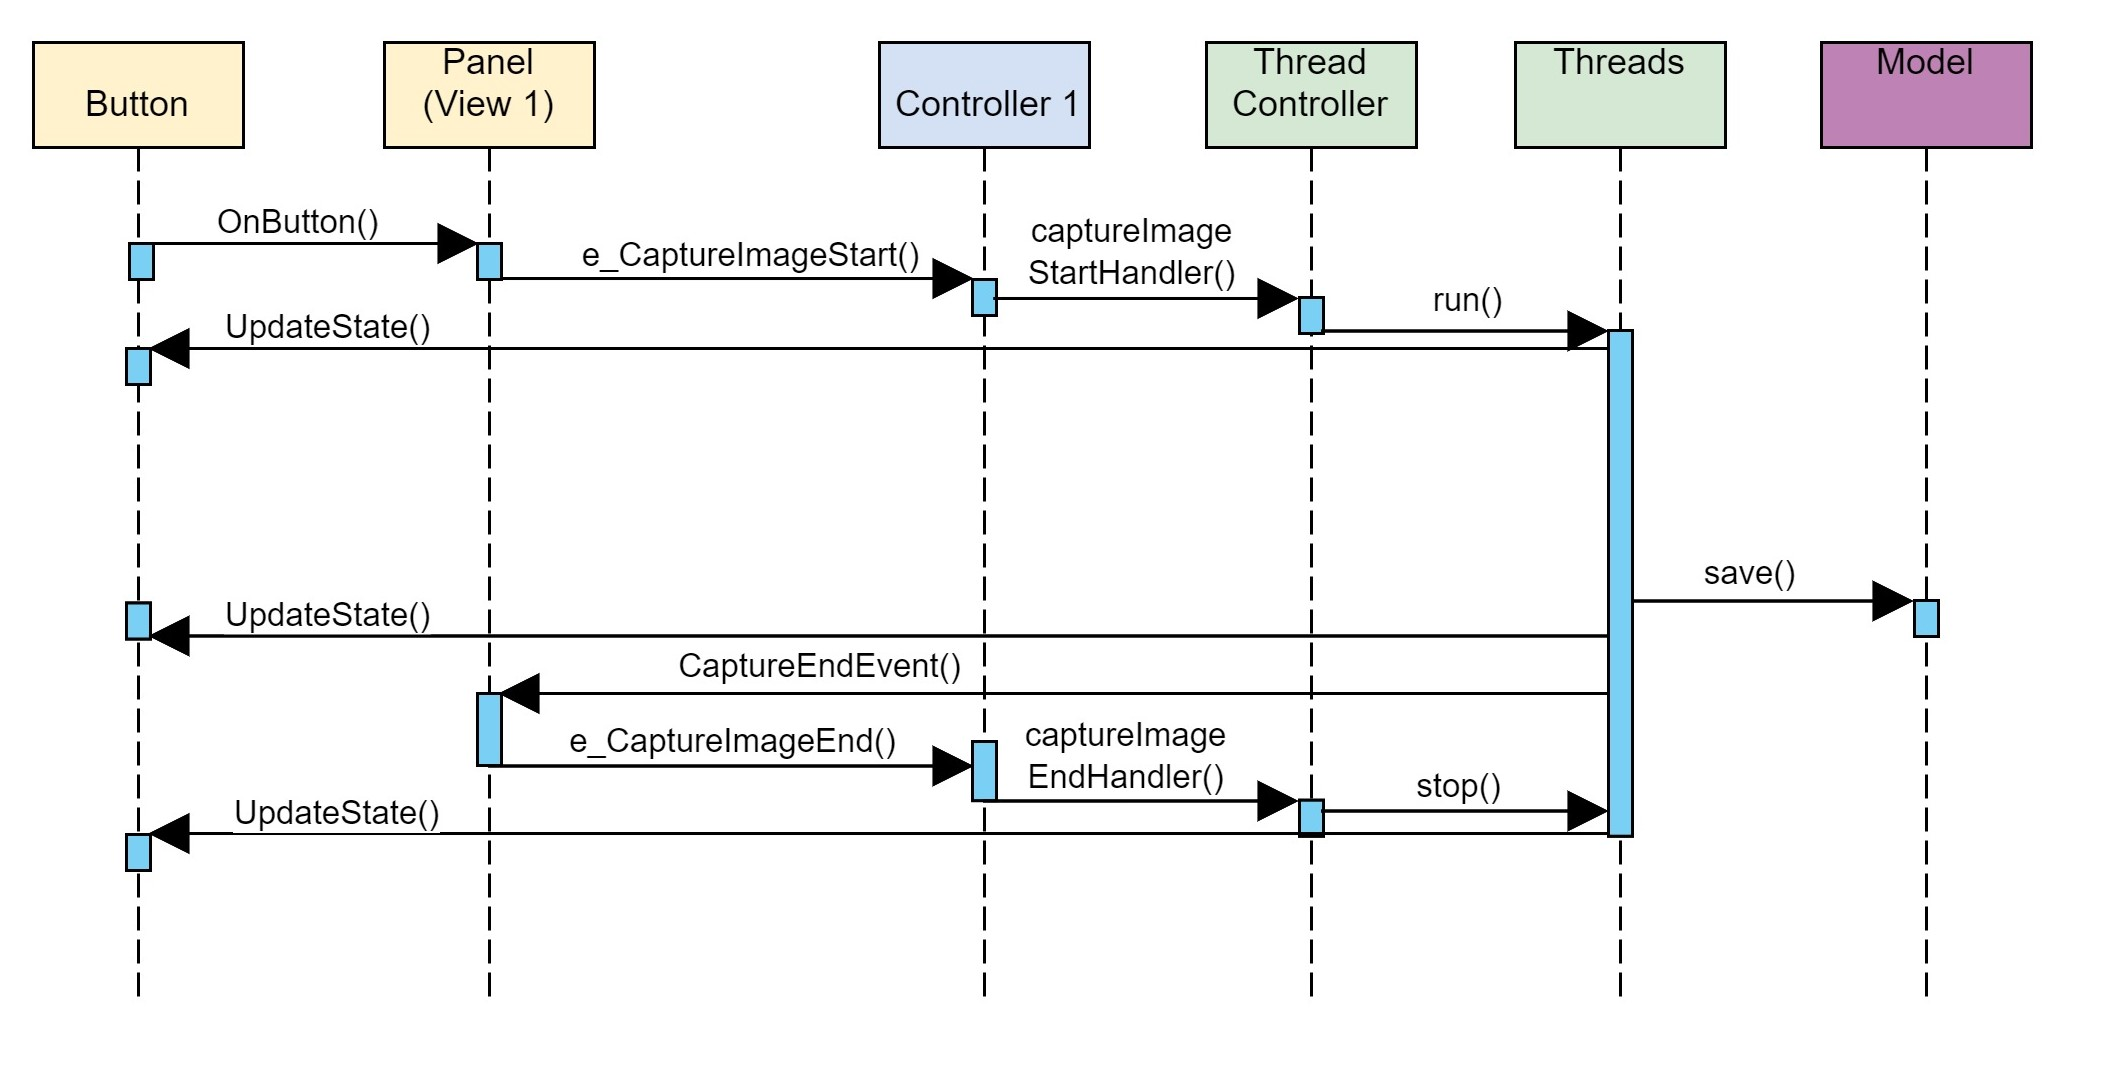
\includegraphics[width=0.9\textwidth]{texs/Part2/chapter4/image/sequence.jpg}
    \caption{Example of Request Handling}
    \label{fig:sequence_diagram}
\end{figure}

With this example, the request starts by pressing a button. This action will trigger an event, which will be handled by the \textit{View1}. The View will then request an initialization of process or thread via the endpoint \texttt{e\_CaptureImageStart()}. The request will be forwarded to the \textit{ThreadController}, and a thread to capture the image is initiated and run.

The button state is updated to signal the succession of the request. The thread will run on its own, and when it is finished capturing the image, the data is saved to the Model via the \texttt{save()} method. Once again, The state is updated, and an event signaling the completion of the process is sent to the View.

With this event, the View signals the Controller to stop the thread via the endpoint \texttt{e\_CaptureImageStop()}. The thread is then stopped and joined. The state is updated to signal the completion of the process.

\section{Algorithm Improvement}
\label{sec:algorithm_improvement}

In this section, the improvement of the algorithm is discussed. Based on the previous work \cite{Sabtu_2023}, the algorithm is divided into three main processes: image alignment, object tracking, and distance measurement. Several improvements are made to the algorithm during the implementation process, which are discussed in detail below.

\subsection{Image Alignment}
As per the previous research \cite{Sabtu_2023}, aligning images is carried out by combining feature detection and feature matching algorithms. The feature detection algorithm identifies key points or features between two images, and the matching results are used to calculate the transformation matrix, which aligns the images. The figure below (Figure \ref{fig:image_alignment_process}) illustrates the overall image alignment process.

\begin{figure}[!ht]
    \centering
    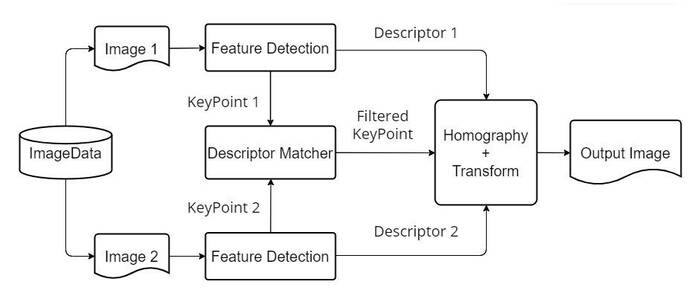
\includegraphics[width=0.9\textwidth]{texs/Part2/chapter4/image/ImageAllignmentAlgoDiagram.jpg}
    \caption{Image Alignment Process}
    \label{fig:image_alignment_process}
\end{figure}

The author has mentioned that the entire process can be pretty time-consuming, especially when dealing with large image sizes. Each step involved in aligning a vector of images of size 1280 x 960 pixels was analyzed to identify the factors contributing to this. Table \ref{table:time_taken} shows the average time taken for each process ($\overline{t_{proc}}$) and the percentage of total time taken ($\%_{total}$). The results indicate that the feature detection process on both reference and target image is the most time-consuming, accounting for up to 95\% of the overall process.

\begin{table}[!ht]
    \centering
    \begin{tabular}{|l|r|r|}
        \hline
        \textbf{Process}                     & \textbf{$\overline{t_{proc}}$ [ms]} & \textbf{$\%_{total}$ [\%]} \\ \hline
        Feature detection on reference image & 1579.92                             & 47.827                     \\ \hline
        Feature detection on targe image     & 1582.64                             & 47.909                     \\ \hline
        Feaure Matching                      & 101.27                              & 3.066                      \\ \hline
        Filter Keypoints                     & 0.30                                & 0.009                      \\ \hline
        Homography                           & 2.27                                & 0.069                      \\ \hline
        Transform                            & 37.01                               & 1.120                      \\ \hline
    \end{tabular}
    \caption{Time taken for each process}
    \label{table:time_taken}
\end{table}


After further analysis of the process, it has been determined that performing feature detection on the reference image is unnecessary for every iteration. In this context, the reference image refers to the first image to which we want to align the other images. Therefore, feature detection on the reference image only needs to be done once, and the resulting data can be cached and used for subsequent iterations. Implementing this approach will significantly reduce the time taken for the feature detection process and the overall processing time.

Figure \ref{fig:image_alignment_process_with_caching} illustrates the image alignment process with caching. In this process, the output of feature detection on the reference image is stored in a cache and used in subsequent iterations. Table \ref{table:time_taken_improvement} presents the average time taken for aligning the image ($\overline{t_{align}}$) using different implementations. It also shows the percentage of improvement relative to the original implementation ($\%_{improve}$). As per the results, the improved implementation is approximately 93\% faster than the original implementation.

\begin{figure}[ht!]
    \centering
    \begin{subfigure}[c]{0.8\textwidth}
        \begin{minipage}{\textwidth}
            \centering
            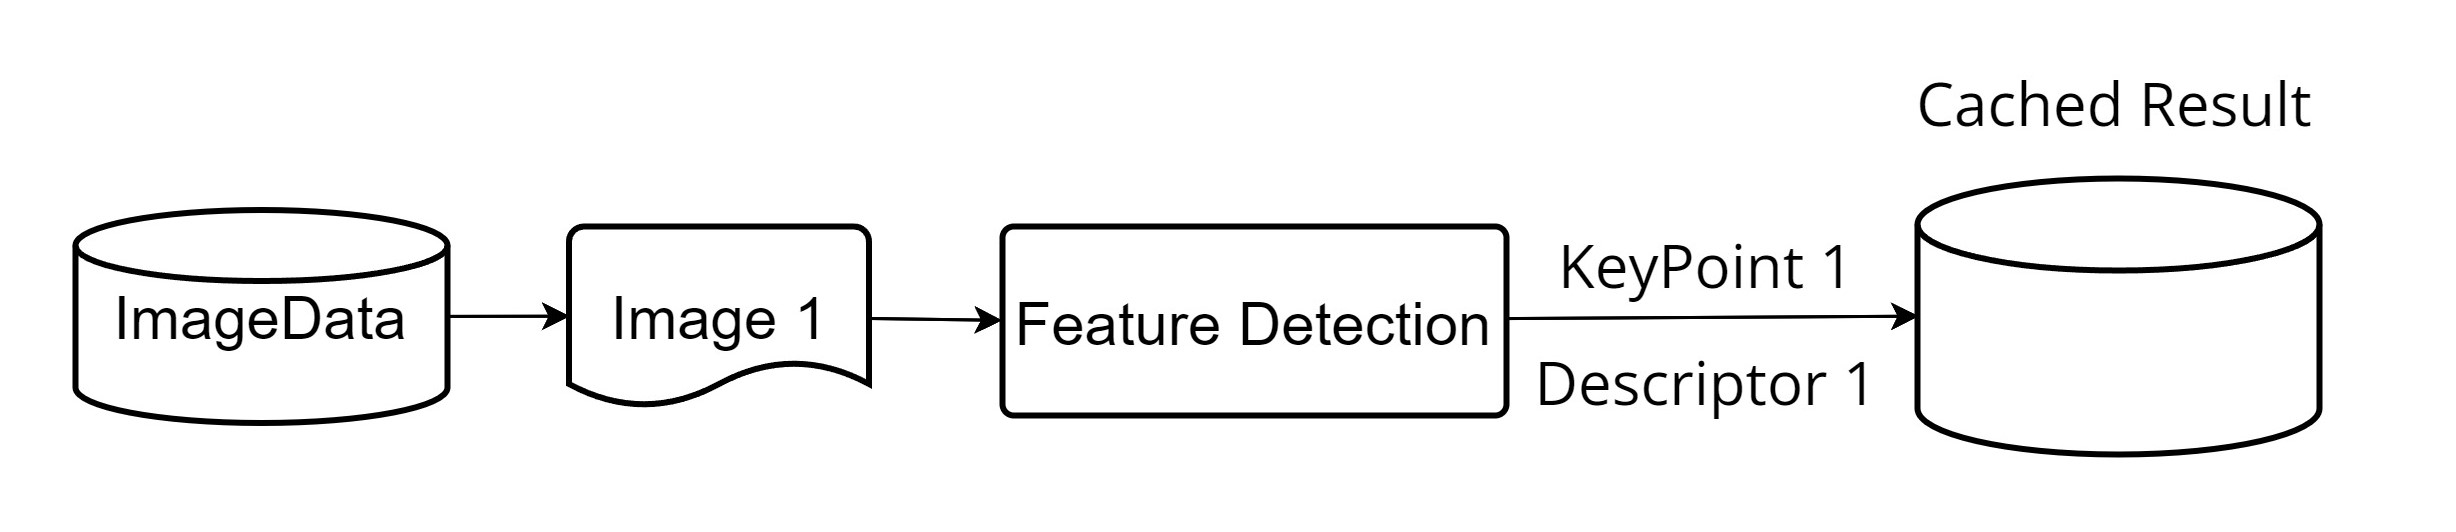
\includegraphics[width=0.8\textwidth]{texs/Part2/chapter4/image/fea1.jpg}
        \end{minipage}
        \caption{Caching the result of feature detection on reference image}
        \label{fig:improve_cache}
    \end{subfigure}
    % \hfill
    \begin{subfigure}[c]{0.8\textwidth}
        \begin{minipage}{\textwidth}
            \centering
            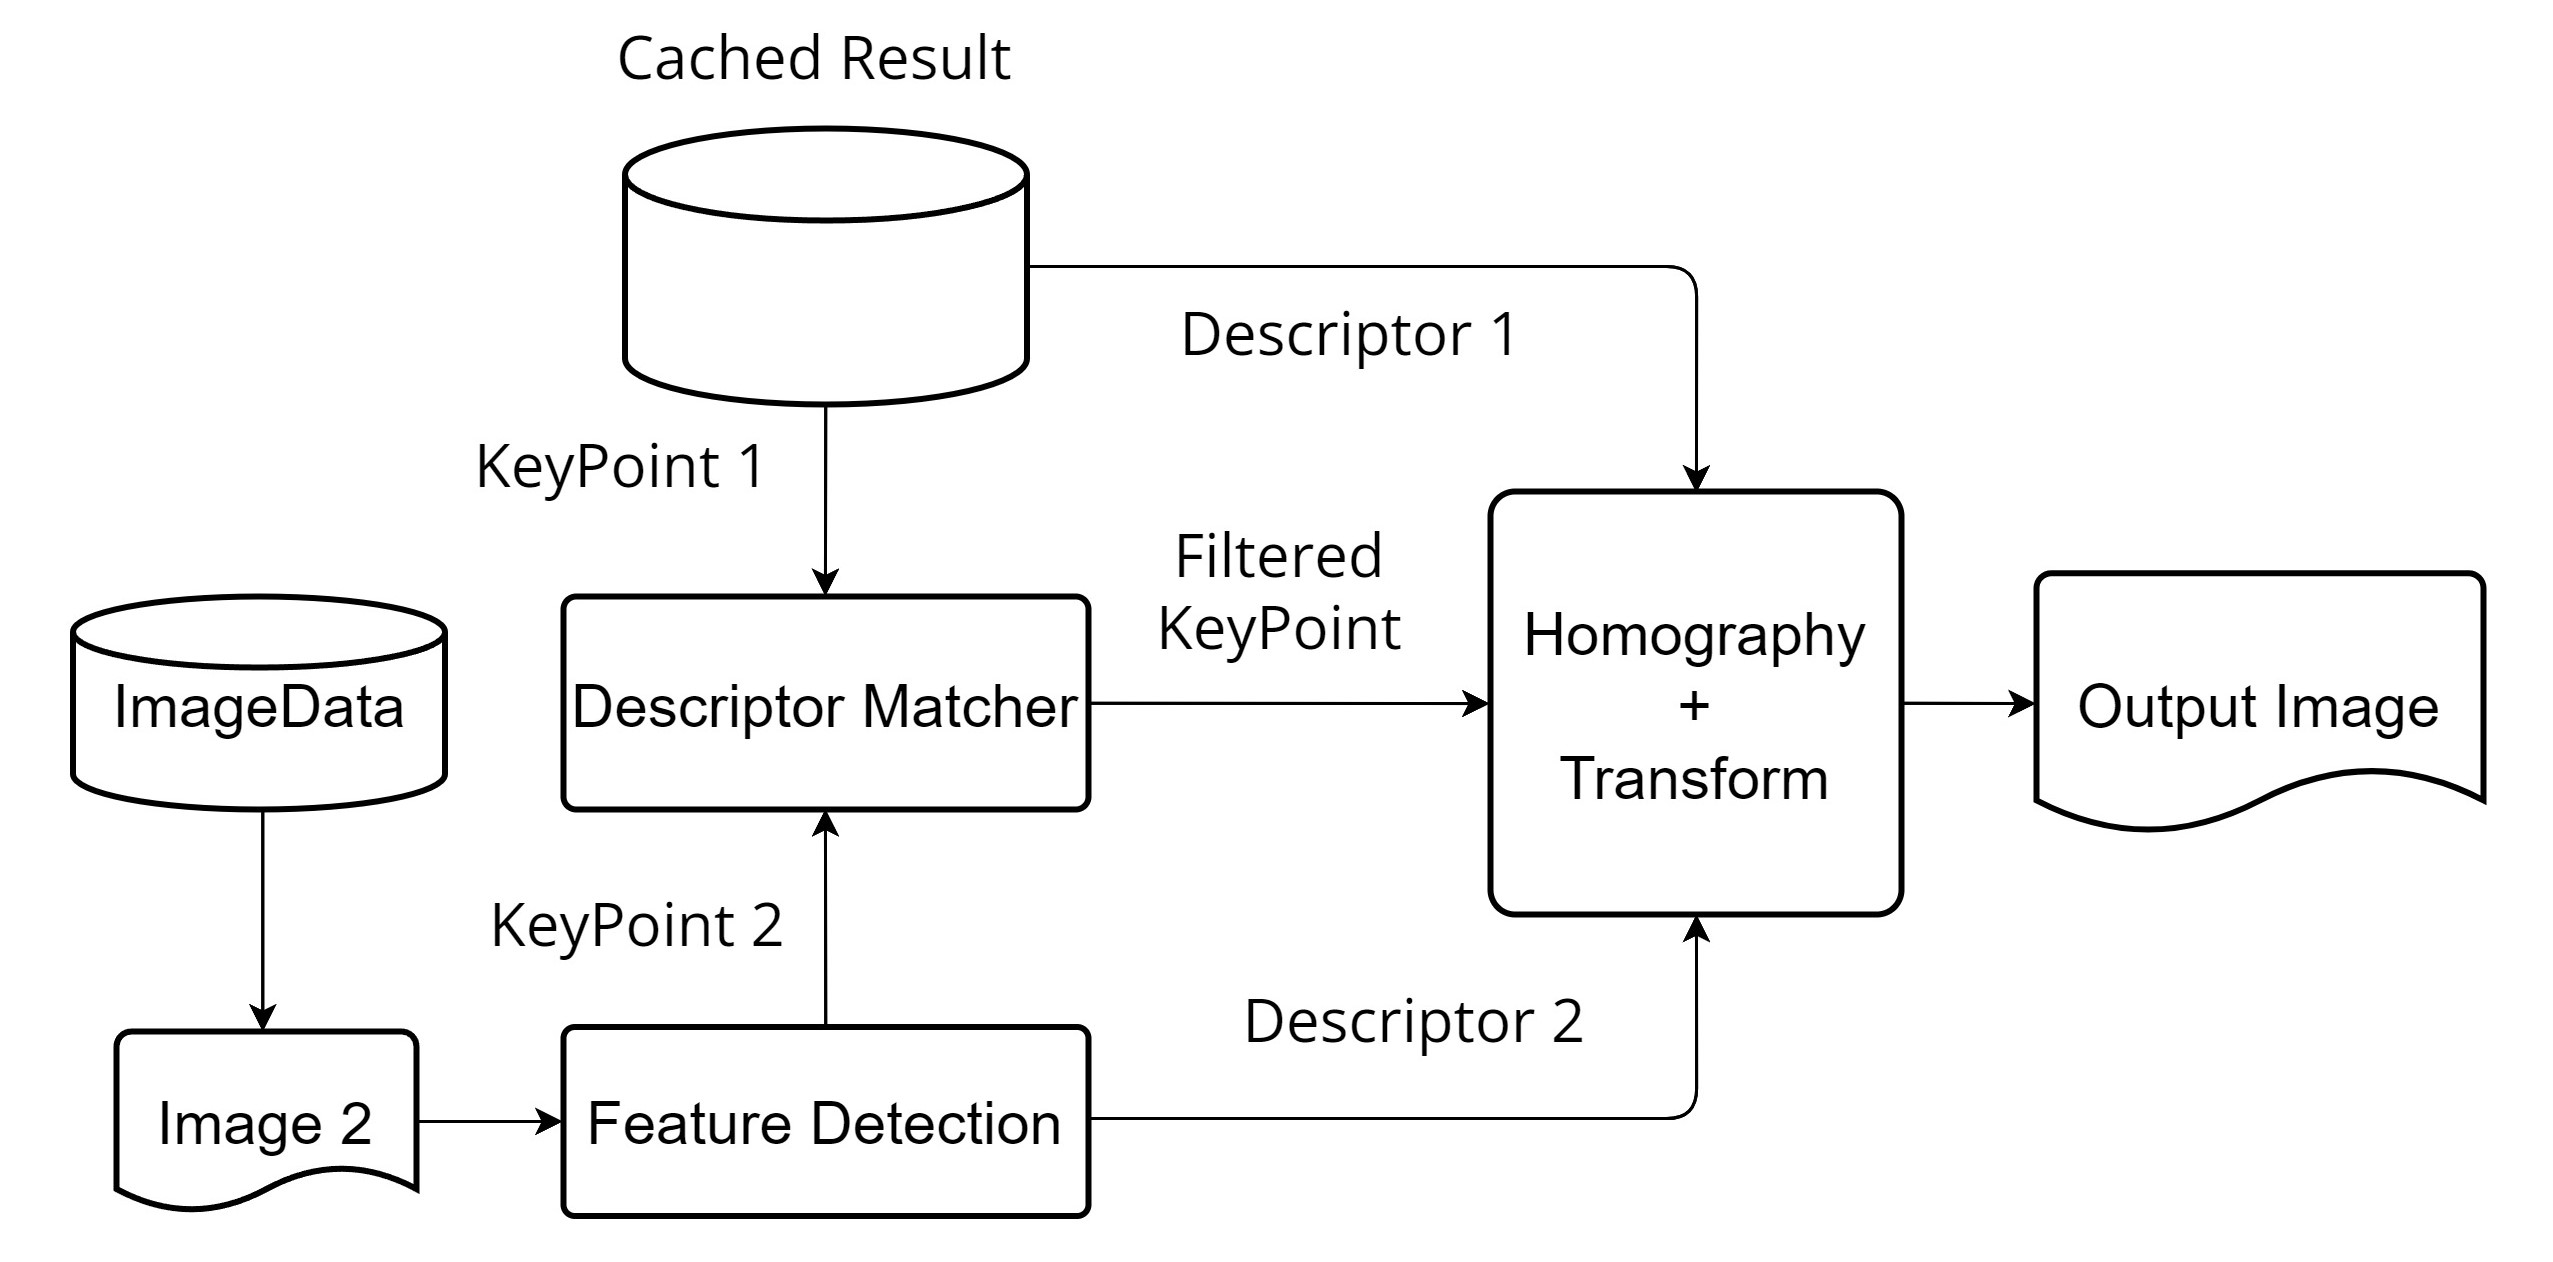
\includegraphics[width=0.8\textwidth]{texs/Part2/chapter4/image/fea2.jpg}
        \end{minipage}
        \caption{Aligning the image using cached result}
        \label{fig:improve_align}
    \end{subfigure}
    \caption{Image Alignment Process with Caching}
    \label{fig:image_alignment_process_with_caching}
\end{figure}

\begin{table}[!ht]
    \centering
    \begin{tabular}{|l|r|r|}
        \hline
        \textbf{Implementation Type} & \textbf{$\overline{t_{align}}$ [ms]} & \textbf{$\%_{improve}$ [\%]} \\ \hline
        Original                     & 3160                                 & 0                            \\ \hline
        Cached                       & 1631                                 & 93.7                         \\ \hline
        Cached + 2 Workers           & 1085                                 & 191.2                        \\ \hline
        Cached + 3 Workers           & 941                                  & 235.8                        \\ \hline
    \end{tabular}
    \caption{Comparison of time taken for image alignment}
    \label{table:time_taken_improvement}
\end{table}

In addition, by using a thread pool as described in section \ref{subsec:thread-pool}, the process can be enhanced even more by utilizing parallel execution. Table \ref{table:time_taken_improvement} illustrates that with 2 and 3 workers, the process can be improved by 191.2 \% and 235.8 \%, respectively.


\subsection{Custom Lane}
\label{subsec:custom_lane}
According to a previous study \cite{Sabtu_2023}, measuring the distance of an object from the camera requires knowledge of the distance between the two lanes on the road. Typically, in Germany, this distance is around 3.5 meters. However, in real-world situations, this distance may vary, leading to measurement inaccuracies. The study also highlights the importance of accurately selecting the lane representing the distance between the two lanes. Even a slight error in lane selection can result in a significant measurement error.

A simplified method has been introduced to streamline the selection of the appropriate line. This method introduces a custom object with predetermined dimensions into the camera's field of view, serving as a reference point (as depicted in Figure \ref{fig:custom_object}). This object includes two lines, one in blue and the other in yellow. Both lines run parallel and are precisely 420 mm apart and will serve as references for the measurement procedure. An illustration of the line selection process can be seen in Figure \ref{fig:select_lines}.

\begin{figure}[!ht]
    \centering
    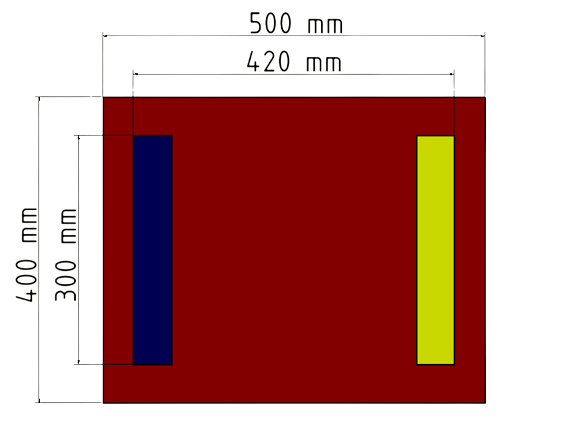
\includegraphics[width=0.6\textwidth]{texs/Part2/chapter4/image/matdimension.png}
    \caption{Custom Object}
    \label{fig:custom_object}
\end{figure}

\begin{figure}[!ht]
    \centering
    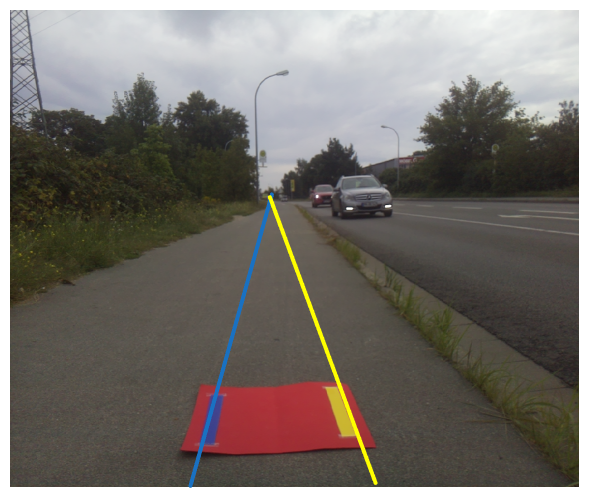
\includegraphics[width=0.4\textwidth]{texs/Part2/chapter4/image/mat2.png}
    \caption{Example of selecting lines for measurement}
    \label{fig:select_lines}
\end{figure}

\subsection{Distance Measurement}
\label{subsec:distance_measurement}

Distance measurement is based on Javadi et al.'s work \cite{Javadi2019}. This type of speed measurement will serve as an alternative speed calculation method to lane measurement for this research.

To accurately determine the speed of a tracked object, a series of steps must be taken. First, a known object of a specific length should be positioned within the camera's view to serve as a reference point. This reference object will aid in calculating the speed of the tracked object. Next, two lines should be drawn to mark the starting and ending points of the placed object. An illustration of this process can be observed in Figure \ref{fig:distance_measurement_process}.

\begin{figure}[ht!]
    \centering
    \begin{subfigure}[c]{0.8\textwidth}
        \begin{minipage}{\textwidth}
            \centering
            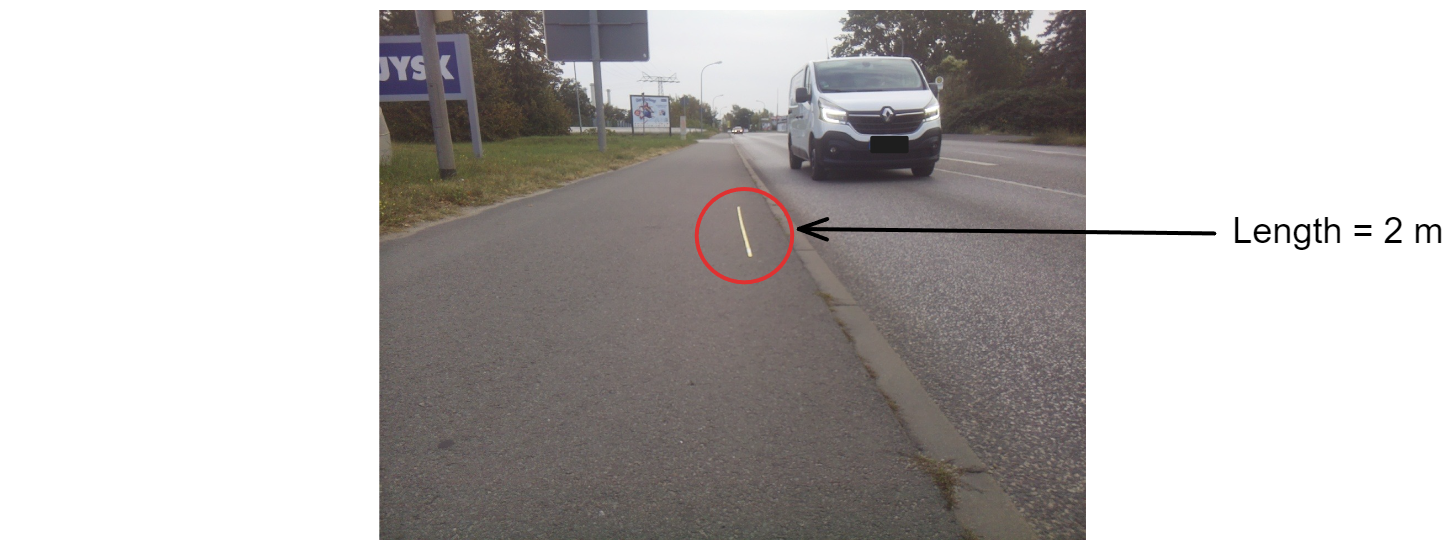
\includegraphics[width=0.8\textwidth]{texs/Part2/chapter4/image/dist1.png}
        \end{minipage}
        \caption{Placement of reference object}
        \label{fig:dist_placement}
    \end{subfigure}
    % \hfill
    \begin{subfigure}[c]{0.8\textwidth}
        \begin{minipage}{\textwidth}
            \centering
            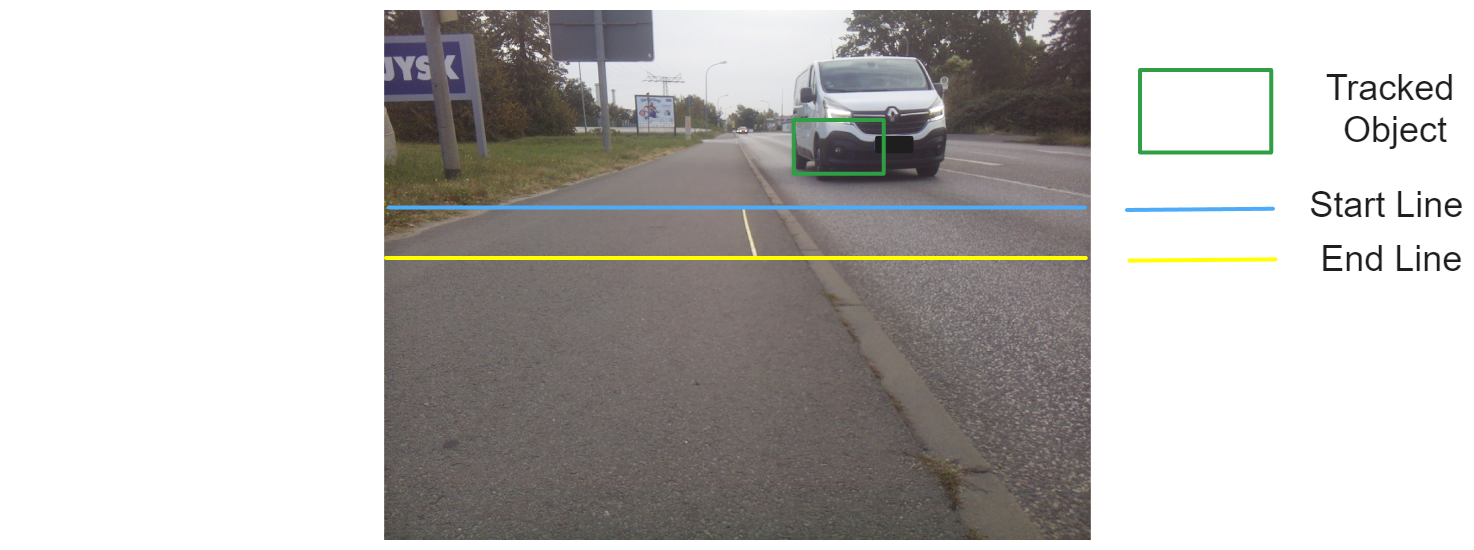
\includegraphics[width=0.8\textwidth]{texs/Part2/chapter4/image/dist2.png}
        \end{minipage}
        \caption{Calibration of Start and End Line}
        \label{fig:dist_calibration}
    \end{subfigure}
    \caption{Distance Measurement Process}
    \label{fig:distance_measurement_process}
\end{figure}

By tracking an object's movement, we can determine the frame at which it crosses both the start and end lines. This allows us to calculate the time it crossed the start line ($t_{start}$) and the time it crossed the end line ($t_{end}$). With the length of the object ($l_{object}$) already known, we can estimate its speed using the following formula:

\begin{equation}
    Speed = \frac{l_{object}}{t_{end} - t_{start}}
\end{equation}

Compared to the lane measurement method, this method is more straightforward. However, as mentioned by Javadi et al. \cite{Javadi2019}, it may lead to inaccurate calculations as the exact time of the object crossing the start and end lines cannot be precisely determined.

This measurement method is implemented in \texttt{DistSpeedMeasurement} class. Please refer to the project documentation on \ref{appendix:documentation} for more information.
















